% Public source snapshot: implementation blocks whose provenance overlaps with
% Dive into Deep Learning (D2L), or whose independent provenance could not be
% established, have been omitted. See sources/README.md for the project's
% stricter independent-provenance and licensing boundary.
\documentclass{article}
\usepackage{graphicx}
\usepackage{amsmath}
\usepackage{amssymb}
\usepackage[margin=1in]{geometry}
\usepackage{xcolor}
\usepackage{tikz}
\usetikzlibrary{shapes, arrows, positioning, calc}
\usepackage{tcolorbox}
\usepackage{booktabs}

\title{Lecture 10: Vision Transformers -- From Sequences to Images}
\author{Deep Learning Class}
\date{\today}

\begin{document}
\maketitle

\section{Introduction: The Journey from Machine Translation to Computer Vision}

In our previous lectures, we explored how Transformers revolutionized sequence-to-sequence learning in machine translation. The key innovation was replacing RNN encoders with the Transformer encoder, which brings:

\begin{itemize}
\item \textbf{No recurrence}: All token interactions happen via attention
\item \textbf{Parallelizable computation}: No sequential dependencies
\item \textbf{Global context}: Each token attends to all other tokens
\item \textbf{Better gradient flow}: Direct connections enable training of deeper models
\end{itemize}

This raises a natural question: \textit{Can we apply the same architectural principles to computer vision?}

The answer is yes. The first major work to do this successfully was ``An Image is Worth 16x16 Words: Transformers for Image Recognition at Scale'' (Dosovitskiy et al., 2021), which introduced the \textbf{Vision Transformer (ViT)}.

The authors' approach was a \textbf{deliberately minimal transplant from NLP}. They kept the vanilla Transformer encoder unchanged and simply modified the input, treating images as sequences of patches. This architectural simplicity is the entire point -- if it works, we have found a truly universal architecture.

\subsection{From Sequence-to-Sequence to Encoder-Only: A Key Architectural Shift}

Before we dive into Vision Transformers, we need to understand an important architectural pattern that we have not yet explored in depth.

\paragraph{What we have seen so far:} In machine translation, we used the complete Transformer architecture:
\begin{itemize}
\item \textbf{Encoder}: Processes the source sentence and creates contextualized representations
\item \textbf{Decoder}: Generates the target sentence one token at a time, attending to the encoder's output
\item \textbf{Task}: Sequence-to-sequence generation (French $\rightarrow$ English)
\end{itemize}

\paragraph{A new paradigm: Encoder-only for classification.} For many tasks, we do not need to \textit{generate} a sequence -- we just need to \textit{understand} and \textit{classify} the input. Examples include:
\begin{itemize}
\item Sentiment analysis: Is this movie review positive or negative?
\item Image classification: Does this image contain a cat or a dog?
\item Document categorization: What topic does this article belong to?
\end{itemize}

For these tasks, we can use \textbf{only the encoder} part of the Transformer:

\begin{figure}[h]
\centering
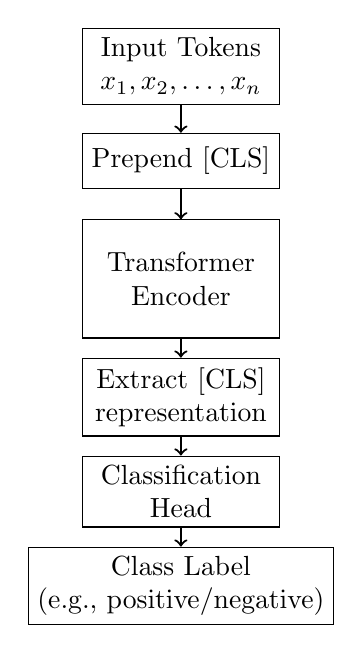
\begin{tikzpicture}[
    node distance=1.2cm,
    box/.style={rectangle, draw, minimum width=2.5cm, minimum height=0.7cm, align=center},
    bigbox/.style={rectangle, draw, minimum width=2.5cm, minimum height=1.5cm, align=center}
]

% Input tokens
\node[box] (input) {Input Tokens\\$x_1, x_2, \ldots, x_n$};

% Add special token
\node[box, below of=input] (cls) {Prepend [CLS]};

% Encoder
\node[bigbox, below of=cls, yshift=-0.3cm] (encoder) {Transformer\\Encoder};

% Extract CLS
\node[box, below of=encoder, yshift=-0.3cm] (extract) {Extract [CLS]\\representation};

% Classification head
\node[box, below of=extract] (head) {Classification\\Head};

% Output
\node[box, below of=head] (output) {Class Label\\(e.g., positive/negative)};

% Arrows
\draw[->, thick] (input) -- (cls);
\draw[->, thick] (cls) -- (encoder);
\draw[->, thick] (encoder) -- (extract);
\draw[->, thick] (extract) -- (head);
\draw[->, thick] (head) -- (output);

\end{tikzpicture}
\caption{Encoder-only architecture for classification}
\end{figure}

\paragraph{The [CLS] token as a representation.} The key insight is:
\begin{enumerate}
\item We add a special \textbf{[CLS]} (classification) token at the beginning of the input sequence
\item The encoder processes all tokens (including [CLS]) through multiple layers of self-attention
\item Through self-attention, the [CLS] token ``sees'' and aggregates information from all other tokens
\item After the final encoder layer, we extract the [CLS] token's representation
\item We pass this representation through a simple classification head (e.g., a linear layer + softmax)
\end{enumerate}

\begin{tcolorbox}[colback=yellow!5!white, colframe=orange!50!black, title=Why Does This Work?]
The [CLS] token acts as a ``summary vector'' for the entire input sequence. Through the self-attention mechanism:
\begin{itemize}
\item In early layers, [CLS] can attend to all input tokens
\item In later layers, [CLS] has built up a rich representation that captures the relevant information from the entire sequence
\item This representation can be used for classification, just like the final hidden state of an RNN
\end{itemize}

The advantage over RNNs: The [CLS] token has \textit{direct} access to all input tokens via attention, rather than having to propagate information through a sequential bottleneck.
\end{tcolorbox}

\paragraph{From text to images.} This encoder-only pattern is exactly what Vision Transformers use:
\begin{itemize}
\item Instead of word tokens, we have \textbf{image patch tokens}
\item We prepend a [CLS] token to the sequence of patches
\item The Transformer encoder processes all patches
\item We extract the [CLS] representation and classify the image
\end{itemize}

The beautiful simplicity: \textbf{the same architecture that works for text classification also works for image classification}, with only the tokenization strategy changing.

\section{Vision Transformer (ViT) Architecture}

\subsection{From Text Sequences to Image Patches}

\subsubsection{The Core Analogy}

In natural language processing:
\begin{itemize}
\item Input: sequence of word tokens
\item Processing: Transformer encoder creates contextualized representations
\item Output: sequence of enriched token embeddings
\end{itemize}

In computer vision with ViT:
\begin{itemize}
\item Input: sequence of image \textit{patches} (treating patches as ``visual tokens'')
\item Processing: \textit{Same} Transformer encoder architecture
\item Output: sequence of enriched patch embeddings
\end{itemize}

\subsubsection{Patchification Strategy}

Given an image of size $H \times W$ with $C$ channels, we:

\begin{enumerate}
\item Divide the image into non-overlapping patches of size $P \times P$
\item Flatten each patch into a vector of length $C \cdot P^2$
\item This yields $T = \frac{H \cdot W}{P^2}$ patch tokens
\end{enumerate}

For example, a $224 \times 224$ RGB image with patch size $P=16$ gives us:
\begin{equation}
T = \frac{224 \times 224}{16^2} = \frac{50176}{256} = 196 \text{ patches}
\end{equation}

Each patch is a vector of length $3 \times 16^2 = 768$ values.

\subsection{Overall ViT Design}

The ViT architecture consists of three main components:

\begin{enumerate}
\item \textbf{Patch Embedding Layer}: Converts image patches to embedding vectors
\item \textbf{Transformer Encoder}: Stack of self-attention and feed-forward layers
\item \textbf{Classification Head}: Projects the CLS token representation to class logits
\end{enumerate}

\begin{figure}[h]
\centering
\fbox{\textit{[Figure 1 from Dosovitskiy et al., 2021: ViT model overview]}}
\caption{Vision Transformer architecture. The image is split into fixed-size patches, which are linearly embedded. A [CLS] token is prepended, position embeddings are added, and the sequence is fed into a standard Transformer encoder. The [CLS] token output is used for classification. Source: ``An Image is Worth 16x16 Words,'' Figure 1.}
\end{figure}

\begin{figure}[h]
\centering
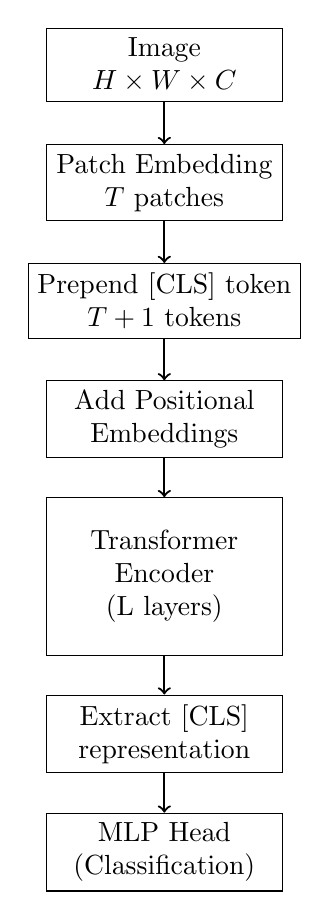
\begin{tikzpicture}[
    node distance=1.5cm,
    box/.style={rectangle, draw, minimum width=3cm, minimum height=0.8cm, align=center},
    bigbox/.style={rectangle, draw, minimum width=3cm, minimum height=2cm, align=center}
]

% Input
\node[box] (input) {Image\\$H \times W \times C$};

% Patch embedding
\node[box, below of=input] (patches) {Patch Embedding\\$T$ patches};

% Add CLS token
\node[box, below of=patches] (cls) {Prepend [CLS] token\\$T+1$ tokens};

% Positional encoding
\node[box, below of=cls] (pos) {Add Positional\\Embeddings};

% Transformer blocks
\node[bigbox, below of=pos, yshift=-0.5cm] (transformer) {Transformer\\Encoder\\(L layers)};

% Extract CLS
\node[box, below of=transformer, yshift=-0.5cm] (extract) {Extract [CLS]\\representation};

% Classification head
\node[box, below of=extract] (head) {MLP Head\\(Classification)};

% Arrows
\draw[->, thick] (input) -- (patches);
\draw[->, thick] (patches) -- (cls);
\draw[->, thick] (cls) -- (pos);
\draw[->, thick] (pos) -- (transformer);
\draw[->, thick] (transformer) -- (extract);
\draw[->, thick] (extract) -- (head);

\end{tikzpicture}
\caption{Vision Transformer pipeline (schematic)}
\end{figure}

\subsection{Detailed Component Breakdown}

\subsubsection{Patch Embedding}

The patch embedding layer can be implemented elegantly as a single convolutional layer:

% [Implementation omitted from the public snapshot: independent provenance could
% not be established.]

The convolution operation with \texttt{kernel\_size = stride = patch\_size} efficiently:
\begin{enumerate}
\item Extracts non-overlapping patches
\item Projects each patch to \texttt{num\_hiddens} dimensions
\end{enumerate}

\subsubsection{The [CLS] Token: A Special Purpose Representation}

The \textbf{classification token} or [CLS] token is the key mechanism for obtaining a fixed-size representation from a variable-length sequence:

\begin{itemize}
\item A learnable embedding prepended to the sequence of patch embeddings
\item Has no correspondence to any image patch
\item Through self-attention, it \textit{aggregates information} from all patches
\item After the Transformer encoder, the [CLS] token representation is used for classification
\end{itemize}

Why use [CLS] instead of averaging all patch representations? The [CLS] token learns to perform \textit{task-specific} aggregation via attention, which is more flexible than simple averaging.

\begin{tcolorbox}[colback=blue!5!white, colframe=blue!50!black, title=Note on [CLS] Token]
The [CLS] token design comes from BERT (Bidirectional Encoder Representations from Transformers) for language modeling. We will see it again when we study BERT in upcoming lectures. It has become a standard design pattern for encoder-only Transformers.
\end{tcolorbox}

\subsubsection{Positional Embeddings}

Self-attention, by its nature, is \textbf{permutation invariant}. If we shuffle the input patches, the output representations will be identical but shuffled in the same way. The model has no inherent knowledge of \textit{where} patch 5 is relative to patch 6.

A CNN knows \textit{exactly} where pixels are due to its kernel-based structure. For ViT, we must explicitly inject this spatial information. This is the sole job of positional embeddings.

The input to the Transformer encoder is:
\begin{equation}
z_0 = [x_{\text{class}}; x_p^1 E; x_p^2 E; \cdots ; x_p^N E] + E_{\text{pos}}
\end{equation}

where $x_p^i$ are the flattened image patches, $E$ is the patch embedding projection, and $E_{\text{pos}}$ are the positional embeddings.

\paragraph{Learnable 1D Embeddings (ViT's Choice):}

The original ViT paper uses the simplest effective solution: a learnable \texttt{nn.Parameter} lookup table.

\begin{itemize}
\item We create a tensor $E_{\text{pos}} \in \mathbb{R}^{(T+1) \times d}$, where $T$ is the number of patches and $d$ is the embedding dimension
\item The $+1$ is for the [CLS] token
\item At initialization, these embeddings carry no information about the 2D positions of the patches
\item During training, the model learns an optimal spatial ``map'' through backpropagation
\item A key finding was that the model learns to encode 2D proximity in this 1D vector -- nearby patches get similar positional embeddings
\end{itemize}

\begin{tcolorbox}[colback=blue!5!white, colframe=blue!50!black, title=Are We Wasting Learning on Already-Known Spatial Proximity?]
A natural question: why use a \textit{learnable} lookup table at all? Aren't we forcing the model to relearn that patch (3,5) is near patch (3,6)?

\paragraph{Why learnable absolute positional embeddings work well:}

\begin{enumerate}
\item \textbf{Self-attention is permutation-invariant}. Without positions, ViT cannot distinguish patch locations at all. The lookup table is the \textit{minimal} injection of spatial information needed.

\item \textbf{Negligible parameter cost}. For ViT-B/16 with $14 \times 14 = 196$ patches plus [CLS], the table has $197 \times 768 = 151{,}296$ parameters -- only 0.17\% of the 86M total model parameters. This tiny overhead buys enormous flexibility.

\item \textbf{Absolute $\rightarrow$ relative cues emerge naturally}. Even with absolute position embeddings, the attention mechanism can infer relative relationships by comparing positions across queries and keys. The model learns to extract whatever geometric relationships help on the training distribution (edges, center bias, etc.) rather than having these hard-coded.

\item \textbf{Patch embedding already provides locality}. The $16 \times 16$ patch projection already mixes local pixels (via convolution), so the model isn't starting completely from scratch on spatial relationships. The positional table complements this by encoding \textit{where} each patch lives in the global image.

\item \textbf{Learned embeddings discover 2D topology}. The ViT authors visualized the learned position embeddings and found that nearby patches in 2D space automatically get similar embeddings, showing the model discovers the grid structure without being told.
\end{enumerate}

\paragraph{Why didn't explicit 2D (row/column) encodings help?}

The original ViT paper experimented with more ``2D-aware'' schemes (e.g., separate embeddings for row and column indices). They found \textbf{no improvement} over the simple learned 1D table.

\textbf{Explanation}: With sufficient data (ImageNet-21k, JFT-300M), the learned 1D embeddings are expressive enough to capture the 2D image grid. Hand-engineering additional structure adds complexity without gains.

\paragraph{When do more structured positional encodings help?}

On \textbf{smaller datasets} or with \textbf{tighter compute budgets}, adding explicit structure can help:
\begin{itemize}
\item \textbf{Relative position bias} (as used in Swin): Encode relative offsets directly in attention
\item \textbf{2D-aware schemes}: Separate row/column embeddings can improve data efficiency
\end{itemize}

Later ViT variants have revisited relative positional encodings and found gains in data-limited regimes where every inductive bias helps.

\paragraph{Bottom line:} The learned lookup table is a cheap, general prior that ViT molds to the data. On large-scale pretraining, it is sufficiently expressive to capture image geometry. On smaller datasets, more structured encodings can help, but aren't necessary with sufficient scale.
\end{tcolorbox}

\subsubsection{Transformer Encoder Block}

The ViT encoder block uses \textbf{pre-normalization} (LayerNorm before attention and MLP):

% [Implementation omitted from the public snapshot: independent provenance could
% not be established.]

\textbf{Why pre-normalization?} In the original ``post-norm'' design ($\text{Norm}(X + \text{Sublayer}(X))$), the output scale can grow rapidly layer by layer, leading to unstable training in very deep models. The ``pre-norm'' design ($X + \text{Sublayer}(\text{Norm}(X))$) provides a ``cleaner'' residual path, which allows gradients to flow more easily and enables stable training of much deeper Transformers.

\subsubsection{MLP Head}

The MLP uses GELU activation instead of ReLU:

% [Implementation omitted from the public snapshot: independent provenance could
% not be established.]

GELU (Gaussian Error Linear Unit) is a smoother activation function than ReLU.

\subsection{Complete ViT Model}

% [Implementation omitted from the public snapshot: D2L-derived material.]

\section{CNN Principles vs. Self-Attention: The Core Trade-off}

\subsection{Inductive Biases in CNNs}

Convolutional Neural Networks are built on two fundamental principles:

\paragraph{Translation Invariance:} A pattern detector should respond the same way regardless of where the pattern appears in the image. Mathematically, if we have a hidden representation $[H]_{i,j}$, the same weights are used regardless of position $(i,j)$:
\begin{equation}
[H]_{i,j} = u + \sum_{\Delta a = -\Delta}^{\Delta} \sum_{\Delta b = -\Delta}^{\Delta} [V]_{a,b} [X]_{i+a,j+b}
\end{equation}

This drastically reduces parameters from $O(H^2 W^2)$ to $O(\Delta^2)$ where $\Delta$ is the kernel size.

\paragraph{Locality:} Only nearby pixels are relevant for computing a feature at position $(i,j)$. We do not need to look at distant regions. This is encoded through finite-sized convolutional kernels (typically $3 \times 3$ or $5 \times 5$).

\subsection{How Transformers Differ}

Vision Transformers take a fundamentally different approach:

\begin{itemize}
\item \textbf{No locality bias}: Self-attention computes interactions between \textit{all pairs} of patches
\item \textbf{No translation invariance}: Position information must be explicitly added via positional encodings
\item \textbf{Content-adaptive}: Attention weights depend on the actual content, not just spatial proximity
\end{itemize}

\subsection{The ViT Scaling Thesis}

This brings us to the core thesis of the original ViT paper.

\begin{tcolorbox}[colback=yellow!5!white, colframe=orange!50!black, title=Key Insight: Inductive Bias vs. Data]
\textbf{CNNs (e.g., ResNet)}: Strong, hand-crafted inductive biases (locality, translation invariance) are ``baked in''. This makes them \textbf{sample efficient} $\rightarrow$ they learn well on small/medium datasets (like ImageNet-1k). However, this fixed prior may limit their capacity.

\textbf{Transformers (ViT)}: Minimal inductive biases. The model must learn spatial relationships from scratch. This makes them \textbf{data-hungry} (they underperform CNNs on small data) but ultimately more \textbf{scalable} $\rightarrow$ given enough data, their flexible, global attention mechanism can outperform fixed convolutional priors.
\end{tcolorbox}

\subsection{Computational Complexity: The Quadratic Bottleneck}

Self-attention has computational complexity $O(T^2 d)$ where:
\begin{itemize}
\item $T = \frac{H \cdot W}{P^2}$ is the number of patches
\item $d$ is the embedding dimension
\end{itemize}

For a $224 \times 224$ image with $P=16$:
\begin{equation}
T = \frac{224 \times 224}{16^2} = 196 \text{ patches}
\end{equation}

This is manageable. But for a $1024 \times 1024$ image:
\begin{equation}
T = \frac{1024 \times 1024}{16^2} = 4096 \text{ patches}
\end{equation}

The attention cost grows as $T^2$, making ViT expensive for high-resolution images.

\section{ViT's Two Major Problems}

The original ViT demonstrated the power of pure self-attention on vision tasks, but exposed two critical limitations:

\begin{enumerate}
\item \textbf{Data Efficiency Problem}: On small/medium datasets (ImageNet-1k, 1.3M images), ViT underperforms CNNs significantly when training from scratch. The lack of inductive biases makes ViT prone to overfitting without massive data.

\item \textbf{Computational Efficiency Problem}: The $O(T^2)$ complexity of global self-attention makes ViT impractical for:
\begin{itemize}
    \item High-resolution images (dense prediction tasks)
    \item Use as a general-purpose backbone for detection/segmentation
    \item Tasks requiring multi-scale feature hierarchies
\end{itemize}
\end{enumerate}

These problems motivated two key extensions: \textbf{DeiT} (Data-efficient Image Transformers) tackled the data efficiency problem, while \textbf{Swin Transformer} tackled the computational efficiency problem. Both approaches fundamentally involve \textit{reintroducing CNN inductive biases}, but in different ways.

This leads us to our organizing framework for understanding how to make ViTs practical.

\section{A Three-Door Taxonomy: Incorporating CNN Inductive Bias into ViTs}

Before diving into specific models, let us establish a conceptual framework. There are three fundamentally different ways to inject CNN-like inductive biases into Vision Transformers:

\begin{figure}[h]
\centering
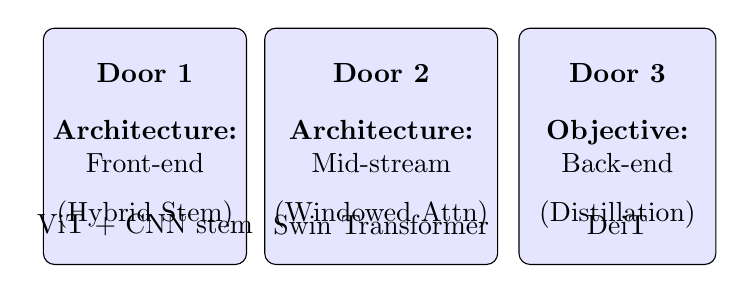
\begin{tikzpicture}[
    node distance=3cm,
    door/.style={rectangle, draw, rounded corners, minimum width=2.5cm, minimum height=3cm, align=center, fill=blue!10},
    arrow/.style={->, thick}
]

% Three doors
\node[door] (door1) {\textbf{Door 1}\\[0.3cm]\textbf{Architecture:}\\Front-end\\[0.2cm](Hybrid Stem)};
\node[door, right of=door1] (door2) {\textbf{Door 2}\\[0.3cm]\textbf{Architecture:}\\Mid-stream\\[0.2cm](Windowed Attn)};
\node[door, right of=door2] (door3) {\textbf{Door 3}\\[0.3cm]\textbf{Objective:}\\Back-end\\[0.2cm](Distillation)};

% Labels below
\node[below of=door1, yshift=2cm] {ViT + CNN stem};
\node[below of=door2, yshift=2cm] {Swin Transformer};
\node[below of=door3, yshift=2cm] {DeiT};

\end{tikzpicture}
\caption{Three ways to incorporate CNN inductive biases into Vision Transformers}
\end{figure}

\subsection{Door 1: Architecture -- Front-End Features (Hybrid ViT)}

\textbf{Core Idea}: Replace raw patch embedding with features from a shallow CNN stem.

\paragraph{What is injected:} Locality, approximate translation equivariance, weight sharing.

\paragraph{Where:} \textit{Input pipeline} -- a shallow convolutional stem (e.g., first few layers of ResNet) produces feature maps before patchifying.

\paragraph{How it works:}
\begin{enumerate}
\item Feed image through a shallow CNN (e.g., ResNet Stage 1-2)
\item Extract intermediate feature maps (e.g., $14 \times 14 \times 256$)
\item Treat each spatial location as a ``patch'' (possibly $1 \times 1$)
\item Feed these CNN features into the standard Transformer encoder
\end{enumerate}

\paragraph{Effect:}
\begin{itemize}
\item Improves optimization and data efficiency on small datasets
\item Preserves global self-attention in later layers
\item The CNN extracts low-level features (edges, textures); Transformer handles high-level reasoning
\end{itemize}

\paragraph{Trade-offs:}
\begin{itemize}
\item Adds FLOPs only at the very front (minimal overhead)
\item Keeps global receptive field in Transformer layers
\item Reintroduces some architectural complexity
\end{itemize}

\begin{figure}[h]
\centering
\fbox{\textit{[Figure from WACV'23 ``Boosting Vision Transformers for Image Retrieval'': Hybrid stem]}}
\caption{Hybrid ViT with CNN stem. The CNN backbone extracts feature maps which are then tokenized and fed to the Transformer encoder. Source: Shen et al., WACV 2023, Figure 1.}
\end{figure}

\paragraph{When to use:}
\begin{itemize}
\item Training on small/medium datasets without strong data augmentation
\item Want benefits of global attention but need better convergence
\item Minimal redesign -- easy plug-in to existing ViT code
\end{itemize}

\subsection{Door 2: Architecture -- Mid-Stream Computation (Swin Transformer)}

\textbf{Core Idea}: Constrain how information flows \textit{inside} the model through windowed attention and hierarchical structure.

\paragraph{What is injected:} Locality + hierarchy (multi-scale pyramids via patch merging), limited receptive field per block.

\paragraph{Where:} \textit{Inside the model} -- windowed attention (W-MSA) and shifted windows (SW-MSA) enforce local interactions while allowing cross-window communication over depth.

\paragraph{How it works:} (Details in Section~\ref{sec:swin})
\begin{enumerate}
\item Compute self-attention only within local $M \times M$ windows (e.g., $7 \times 7$)
\item Alternate between regular and shifted window partitions across layers
\item Use patch merging to create hierarchical, multi-scale features
\end{enumerate}

\paragraph{Effect:}
\begin{itemize}
\item Linear-time scaling with image size: $O(hwM^2C)$ vs. $O((hw)^2C)$
\item Naturally multi-scale, great for detection/segmentation/high-resolution
\item Builds global context gradually through depth
\end{itemize}

\paragraph{Trade-offs:}
\begin{itemize}
\item Global context is built gradually (depth matters more)
\item Design choices (window size, shift amount) become hyperparameters
\item More complex implementation than vanilla ViT
\end{itemize}

\paragraph{When to use:}
\begin{itemize}
\item High-resolution images or dense prediction tasks
\item Need hierarchical features for detection/segmentation
\item Computational efficiency is critical
\end{itemize}

\subsection{Door 3: Objective/Training Signal (DeiT)}

\textbf{Core Idea}: Inject CNN priors via \textit{targets}, not architecture -- a CNN teacher guides training.

\paragraph{What is injected:} CNN decision boundaries and feature preferences via soft targets.

\paragraph{Where:} \textit{Loss/heads} -- a distillation token and head learn to match a CNN teacher's predictions.

\paragraph{How it works:} (Details in Section~\ref{sec:deit})
\begin{enumerate}
\item Add a learnable distillation token (like [CLS])
\item Train with three losses:
    \begin{itemize}
    \item [CLS] token supervised by true labels
    \item Distillation token supervised by CNN teacher predictions
    \item KL divergence between distillation token and teacher
    \end{itemize}
\item At inference, average [CLS] and distillation token outputs
\end{enumerate}

\paragraph{Effect:}
\begin{itemize}
\item Strong gains in data-scarce settings (ImageNet-1k) without constraining model expressivity
\item ``Softly'' imports CNN priors -- the distillation token learns features aligned with convolutional biases
\item Combined with strong augmentation (RandAugment, Mixup, CutMix), achieves CNN-level performance
\end{itemize}

\paragraph{Trade-offs:}
\begin{itemize}
\item Needs a good teacher and carefully tuned training recipe
\item Bias strength depends on teacher quality
\item Extra token only during training/inference
\end{itemize}

\paragraph{When to use:}
\begin{itemize}
\item Small/medium datasets (ImageNet-1k from scratch)
\item Want pure Transformer architecture but need better data efficiency
\item Have access to a strong CNN teacher
\end{itemize}

\subsection{Unifying View: Three Axes}

\begin{table}[h]
\centering
\begin{tabular}{lccc}
\toprule
\textbf{Axis} & \textbf{Hybrid ViT} & \textbf{Swin} & \textbf{DeiT} \\
\midrule
\textbf{Explicitness} & Hard-coded & Hard-coded & Soft/learned \\
\textbf{Where applied} & Input (front) & Internal (mid) & Objective (back) \\
\textbf{Property} & Locality + equiv. & Locality + hierarchy & Teacher-shaped \\
\textbf{Complexity} & $O(N)$ global attn & $O(N)$ windowed & $O(N^2)$ global attn \\
\textbf{Best for} & Stable training & High-res/dense & Small data \\
\bottomrule
\end{tabular}
\caption{Comparison of three approaches to incorporating CNN biases}
\end{table}

\begin{tcolorbox}[colback=green!5!white, colframe=green!50!black, title=Teaching Metaphor]
Think of training a ViT as entering a building:

\begin{itemize}
\item \textbf{Front-door bias (Hybrid ViT)}: Curate what the model ``sees'' first -- give it pre-processed CNN features
\item \textbf{Hallway rules (Swin)}: Constrain how information flows inside -- enforce locality through windowed attention
\item \textbf{Back-door coaching (DeiT)}: A seasoned CNN teacher whispers the answers during training
\end{itemize}
\end{tcolorbox}

\section{Door 3 in Detail: DeiT (Data-Efficient Image Transformers)}
\label{sec:deit}

\textbf{Paper}: ``Training data-efficient image transformers \& distillation through attention'' (Touvron et al., 2021)

\textbf{Motivation}: The original ViT required pretraining on massive datasets (JFT-300M, 300M images) to outperform CNNs. DeiT asks: \textit{Can we make ViT competitive when trained only on ImageNet-1k (1.3M images) using commodity hardware?}

\subsection{The Training Recipe: Strong Augmentation \& Regularization}

ViTs, lacking inductive bias, are prone to overfitting on small datasets. DeiT counters this with an aggressive cocktail of data augmentation and regularization:

\begin{table}[h]
\centering
\begin{tabular}{ll}
\toprule
\textbf{Technique} & \textbf{Purpose} \\
\midrule
RandAugment & Random augmentation strategies \\
CutMix \& Mixup & Blend training examples \\
Random Erasing & Randomly mask rectangular regions \\
Stochastic Depth & Randomly drop layers for regularization \\
Repeated Augmentation & Sample image multiple times with different augs \\
Label Smoothing & Soften hard labels \\
AdamW + Warmup & Optimizer with cosine decay \\
\bottomrule
\end{tabular}
\caption{DeiT's training recipe (adapted from DeiT paper, Table 8)}
\end{table}

\begin{figure}[h]
\centering
\fbox{\textit{[Figure from DeiT paper, Table 8: Training recipe ablation]}}
\caption{Ablation study showing the impact of each augmentation/regularization technique. Each component contributes to closing the gap with CNNs. Source: Touvron et al., 2021, Table 8.}
\end{figure}

This shows that ViTs don't just need \textit{more} data; they need \textit{stronger augmentation} of existing data to learn robustly.

\subsection{Distillation Through Attention: The Key Innovation}

The most clever contribution is a new, Transformer-specific distillation method using a \textbf{distillation token}:

\begin{figure}[h]
\centering
\fbox{\textit{[Figure from DeiT paper, Figure 2: Distillation token architecture]}}
\caption{DeiT architecture with distillation. A learnable distillation token is added alongside the [CLS] token. Both tokens attend to all patches. The [CLS] head is supervised by true labels, while the distillation head is supervised by the teacher's predictions. Source: Touvron et al., 2021, Figure 2.}
\end{figure}

\paragraph{Architecture:}
\begin{itemize}
\item Add a new, learnable \textbf{distillation token} to the input (alongside [CLS])
\item Both tokens attend to all patches through self-attention
\item Two separate classification heads:
    \begin{itemize}
    \item \textbf{[CLS] head}: Supervised by ground truth labels (cross-entropy)
    \item \textbf{[Distill] head}: Supervised by teacher's predictions
    \end{itemize}
\item At test time: Outputs from both heads are averaged for final prediction
\end{itemize}

\paragraph{Loss function:}
\begin{align}
\mathcal{L}_{\text{total}} &= (1-\alpha) \mathcal{L}_{\text{CE}}(y, \hat{y}_{\text{cls}}) + \alpha \mathcal{L}_{\text{CE}}(y, \hat{y}_{\text{dist}}) \nonumber \\
&\quad + \beta \mathcal{L}_{\text{KL}}(\hat{y}_{\text{teacher}}, \hat{y}_{\text{dist}})
\end{align}

where $\alpha = 0.5$ and $\beta = 0.5$ are typical values.

\subsection{Why This Works: Softly Importing Inductive Bias}

The distillation token is a brilliant way of ``softly'' importing the inductive biases of a teacher model.

\textbf{Key Finding}: A \textbf{ConvNet teacher (e.g., RegNetY-16GF) is more effective} than a Transformer teacher with similar performance.

\textbf{Why?} The distillation token, interacting with all patch tokens via self-attention, learns to extract features that align with the \textit{convolutional priors} of the teacher. This effectively ``distills'' those valuable biases (locality, translation invariance) into the Transformer's flexible attention patterns.

\subsection{Results and Impact}

\begin{figure}[h]
\centering
\fbox{\textit{[Figure from DeiT paper, Figure 1: Throughput vs. Accuracy comparison]}}
\caption{DeiT achieves competitive accuracy-throughput trade-offs compared to CNNs (ResNets, EfficientNets, RegNets) when trained only on ImageNet-1k. Source: Touvron et al., 2021, Figure 1.}
\end{figure}

\begin{tcolorbox}[colback=yellow!5!white, colframe=orange!50!black, title=DeiT Results on ImageNet-1k]
DeiT-B (Base model, 86M parameters) trained \textbf{only on ImageNet-1k}:
\begin{itemize}
\item Without distillation: 81.8\% top-1 accuracy
\item With distillation from RegNetY-16GF: 83.4\% top-1 accuracy
\item Training time: 3 days on 8 GPUs (vs. weeks on TPU pods for ViT)
\end{itemize}

This made ViT practical for researchers without access to massive datasets or compute.
\end{tcolorbox}

\section{Door 1 in Detail: Hybrid Vision Transformers}

\textbf{Source}: Original ViT paper (Dosovitskiy et al., 2021), Appendix B.1

While the main ViT paper focused on pure patch-based tokenization, the authors also explored \textbf{hybrid models} that use a CNN stem before the Transformer encoder.

\subsection{Architecture}

\begin{figure}[h]
\centering
\fbox{\textit{[Figure from ViT paper or CVPR'24 ``Learning CNN on ViT'': Hybrid architecture]}}
\caption{Hybrid ViT architecture. A shallow CNN extracts feature maps, which are then flattened into a sequence of tokens and fed to the Transformer encoder. Source: ViT paper Appendix / ``Learning CNN on ViT,'' Figure 1.}
\end{figure}

\paragraph{Implementation:}

% [Implementation omitted from the public snapshot: independent provenance could
% not be established.]

\subsection{When Hybrids Help}

From the ViT paper's experiments:

\begin{itemize}
\item \textbf{Small datasets}: Hybrids outperform pure ViT on small/medium datasets
\item \textbf{Very small patch sizes}: For pure ViT with $P=1$ (pixel-level), performance is poor; hybrid with $P=1$ works well
\item \textbf{Large-scale pretraining}: The gap narrows -- with JFT-300M pretraining, pure ViT catches up to hybrids
\end{itemize}

\textbf{Interpretation}: The CNN stem provides useful inductive biases that help optimization and generalization on limited data. With enough data, ViT can learn these biases, making the hybrid less necessary.

\subsection{Practical Recommendation}

\begin{tcolorbox}[colback=blue!5!white, colframe=blue!50!black, title=When to Use Hybrid ViT]
Use hybrid ViT when:
\begin{itemize}
\item Training from scratch on small/medium datasets
\item Want to leverage existing CNN checkpoints
\item Need better convergence without extensive hyperparameter tuning
\item Don't have resources for DeiT-style heavy augmentation
\end{itemize}

Stick with pure ViT when:
\begin{itemize}
\item Fine-tuning from large-scale pretrained checkpoints
\item Have sufficient data and compute for proper training
\item Want architectural simplicity and universality
\end{itemize}
\end{tcolorbox}

\section{Door 2 in Detail: Swin Transformer}
\label{sec:swin}

\textbf{Paper}: ``Swin Transformer: Hierarchical Vision Transformer using Shifted Windows'' (Liu et al., 2021)

\textbf{Motivation}: ViT (and DeiT) still suffer from two architectural limitations:
\begin{enumerate}
\item \textbf{Quadratic cost}: Global attention $O(T^2)$ is infeasible for high-resolution images
\item \textbf{Single scale}: ViT outputs fixed-resolution features, unlike CNNs' pyramidal features needed for detection/segmentation
\end{enumerate}

Swin solves both by reintroducing two CNN priors \textit{into the architecture}: locality (via windows) and hierarchy (via patch merging).

\subsection{Key Ideas}

\subsubsection{Hierarchical Architecture}

Swin builds a multi-scale feature pyramid, just like CNNs:

\begin{figure}[h]
\centering
\fbox{\textit{[Figure from Swin paper, Figure 3: Hierarchical architecture]}}
\caption{Swin Transformer architecture showing four stages with decreasing spatial resolution and increasing channel dimensions. Patch merging layers downsample like pooling in CNNs. Source: Liu et al., 2021, Figure 3a.}
\end{figure}

\begin{itemize}
\item \textbf{Stage 1}: $H/4 \times W/4$ resolution, $C$ channels
\item \textbf{Stage 2}: $H/8 \times W/8$ resolution, $2C$ channels (after patch merging)
\item \textbf{Stage 3}: $H/16 \times W/16$ resolution, $4C$ channels
\item \textbf{Stage 4}: $H/32 \times W/32$ resolution, $8C$ channels
\end{itemize}

\paragraph{Patch Merging:} Combines $2 \times 2$ neighboring patches, concatenates their features, and applies a linear layer to double the channel dimension while halving spatial resolution.

\subsubsection{Windowed Multi-Head Self-Attention (W-MSA)}

Instead of global attention, compute attention within local $M \times M$ windows:

\begin{itemize}
\item Partition feature map into non-overlapping $M \times M$ windows
\item Compute self-attention independently within each window
\item Complexity: $O(M^2 hwC)$ where $M$ is fixed (e.g., 7)
\end{itemize}

\begin{figure}[h]
\centering
\fbox{\textit{[Figure from Swin paper, Figure 1: ViT vs Swin complexity]}}
\caption{ViT's global attention has quadratic complexity in image size, while Swin's windowed attention is linear. This enables scaling to high-resolution images. Source: Liu et al., 2021, Figure 1.}
\end{figure}

\subsubsection{Shifted Window Multi-Head Self-Attention (SW-MSA)}

\textbf{Problem}: Pure windowed attention has no cross-window communication, limiting modeling power.

\textbf{Solution}: Alternate between regular and shifted window partitions:

\begin{figure}[h]
\centering
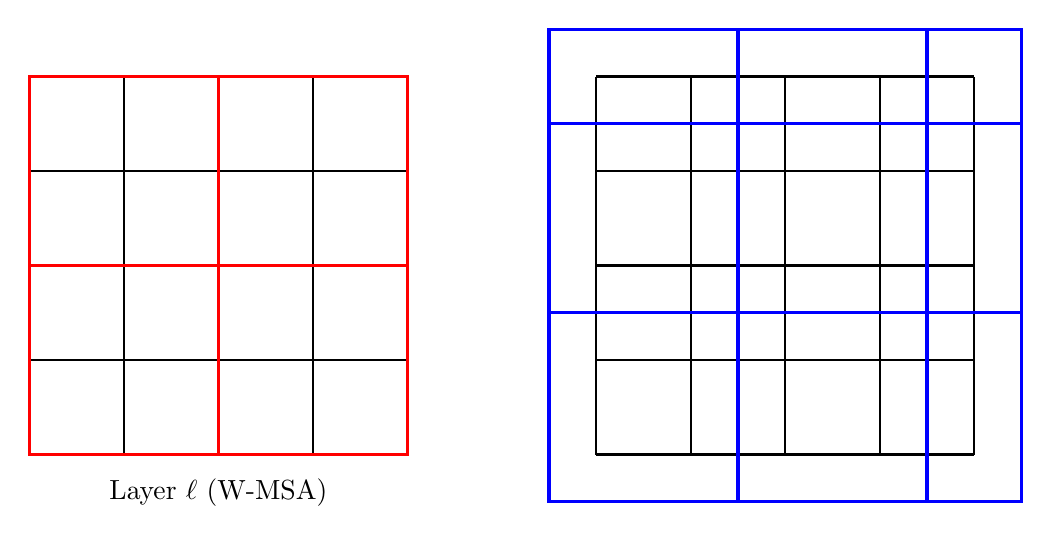
\begin{tikzpicture}[scale=0.6]
% Layer l (regular windows)
\draw[step=2cm, thick] (0,0) grid (8,8);
\draw[very thick, red] (0,0) rectangle (4,4);
\draw[very thick, red] (4,0) rectangle (8,4);
\draw[very thick, red] (0,4) rectangle (4,8);
\draw[very thick, red] (4,4) rectangle (8,8);
\node at (4,-0.8) {Layer $\ell$ (W-MSA)};

% Layer l+1 (shifted windows)
\begin{scope}[xshift=12cm]
\draw[step=2cm, thick] (0,0) grid (8,8);
\draw[very thick, blue] (-1,-1) rectangle (3,3);
\draw[very thick, blue] (3,-1) rectangle (7,3);
\draw[very thick, blue] (7,-1) rectangle (9,3);
\draw[very thick, blue] (-1,3) rectangle (3,7);
\draw[very thick, blue] (3,3) rectangle (7,7);
\draw[very thick, blue] (7,3) rectangle (9,7);
\draw[very thick, blue] (-1,7) rectangle (3,9);
\draw[very thick, blue] (3,7) rectangle (7,9);
\draw[very thick, blue] (7,7) rectangle (9,9);
\clip (0,0) rectangle (8,8);
\draw[very thick, blue] (-1,-1) rectangle (3,3);
\draw[very thick, blue] (3,-1) rectangle (7,3);
\draw[very thick, blue] (7,-1) rectangle (9,3);
\draw[very thick, blue] (-1,3) rectangle (3,7);
\draw[very thick, blue] (3,3) rectangle (7,7);
\draw[very thick, blue] (7,3) rectangle (9,7);
\draw[very thick, blue] (-1,7) rectangle (3,9);
\draw[very thick, blue] (3,7) rectangle (7,9);
\draw[very thick, blue] (7,7) rectangle (9,9);
\node at (4,-0.8) {Layer $\ell+1$ (SW-MSA)};
\end{scope}
\end{tikzpicture}
\caption{Shifted window approach. Regular windows (left) and shifted windows (right) enable cross-window connections.}
\end{figure}

\begin{figure}[h]
\centering
\fbox{\textit{[Figure from Swin paper, Figure 2: Shifted window attention]}}
\caption{Illustration of shifted window partitioning. Windows are shifted by $(\lfloor M/2 \rfloor, \lfloor M/2 \rfloor)$ patches, forcing new windows to straddle boundaries of previous windows. Source: Liu et al., 2021, Figure 2.}
\end{figure}

\begin{itemize}
\item \textbf{Layer $\ell$}: Regular $M \times M$ windows
\item \textbf{Layer $\ell+1$}: Shift windows by $(\lfloor M/2 \rfloor, \lfloor M/2 \rfloor)$ patches
\item This creates cross-window connections while maintaining efficiency
\end{itemize}

\subsection{Complexity Analysis}

Let $h$ and $w$ denote height and width in patches, $C$ the channel dimension.

\textbf{Global MSA (ViT):}
\begin{equation}
\Omega(\text{MSA}) = 4hwC^2 + 2(hw)^2 C
\end{equation}
Quadratic in $hw$ -- doubling resolution increases attention cost by $\sim$4x in spatial term.

\textbf{Windowed MSA (Swin):}
\begin{equation}
\Omega(\text{W-MSA}) = 4hwC^2 + 2M^2 hwC
\end{equation}
Linear in $hw$ since $M$ is fixed -- doubling resolution only doubles attention cost.

\subsection{Relative Position Bias}

Instead of absolute positional embeddings, Swin uses \textbf{relative position bias} $B \in \mathbb{R}^{M^2 \times M^2}$:

\begin{equation}
\text{Attention}(Q, K, V) = \text{SoftMax}\left(\frac{QK^T}{\sqrt{d}} + B\right)V
\end{equation}

The bias $B$ is learned and depends only on relative position offsets between patches within a window.

\subsection{Ablation Study: Proof That It Works}

\begin{table}[h]
\centering
\begin{tabular}{lccc}
\toprule
\textbf{Configuration} & \textbf{ImageNet} & \textbf{COCO} & \textbf{ADE20K} \\
& \textbf{(top-1)} & \textbf{(box AP)} & \textbf{(mIoU)} \\
\midrule
Swin-T (baseline) & 81.3 & 50.5 & 46.1 \\
w/o shifted windows & 80.2 (-1.1) & 47.7 (-2.8) & 43.3 (-2.8) \\
w/ absolute pos. emb. & 80.5 (-0.8) & 49.0 (-1.5) & 43.2 (-2.9) \\
w/o any pos. emb. & 80.1 (-1.2) & 49.2 (-1.3) & 43.8 (-2.3) \\
\bottomrule
\end{tabular}
\caption{Ablation of Swin Transformer design choices (adapted from Liu et al., 2021)}
\end{table}

\textbf{Key Takeaways}:
\begin{enumerate}
\item \textbf{Shifted windows are crucial}: Massive performance drop without them, especially on dense tasks
\item \textbf{Relative position bias wins}: Significantly better than absolute embeddings for all tasks
\end{enumerate}

\subsection{Results and Impact}

Swin Transformer achieved state-of-the-art results across multiple tasks:

\begin{itemize}
\item \textbf{ImageNet-1k}: 87.3\% top-1 (Swin-L)
\item \textbf{COCO object detection}: 58.7 box AP (Swin-L backbone)
\item \textbf{ADE20K semantic segmentation}: 53.5 mIoU (Swin-L backbone)
\end{itemize}

Swin became the \textbf{de facto hierarchical vision backbone}, replacing ResNets in many detection and segmentation frameworks.

\section{When to Use What: Decision Framework}

\begin{table}[h]
\centering
\begin{tabular}{lll}
\toprule
\textbf{Scenario} & \textbf{Recommendation} & \textbf{Reason} \\
\midrule
Small dataset, scratch & Hybrid ViT or DeiT & Front-end or back-end bias \\
ImageNet-1k only & DeiT + strong aug & Data efficiency \\
Large pretrained models & Pure ViT & Scalability \& transfer \\
High-res / dense tasks & Swin & Linear complexity \\
Detection / segmentation & Swin & Hierarchical features \\
Real-time inference & Small Swin or CNN & Efficiency \\
\bottomrule
\end{tabular}
\caption{Decision heuristics for choosing vision architectures}
\end{table}

\subsection{Rules of Thumb}

\begin{enumerate}
\item \textbf{Data size}: $<$100k images from scratch $\Rightarrow$ Hybrid ViT or DeiT; millions or pretrained $\Rightarrow$ ViT
\item \textbf{Resolution / task}: High-res or dense prediction $\Rightarrow$ Swin
\item \textbf{Compute budget}: Limited $\Rightarrow$ Swin or hybrid; ample $\Rightarrow$ large ViT
\item \textbf{Have CNN teacher?}: Yes $\Rightarrow$ DeiT distillation helps
\item \textbf{Patch size}: Larger $P$ $\Rightarrow$ faster but lower accuracy
\end{enumerate}

\section{Experimental Demonstration: Fashion-MNIST}

\subsection{Experimental Setup}

We will train ViT and ResNet-18 on Fashion-MNIST to demonstrate the small-data regime.

\textbf{ViT Configuration:}

% [Implementation omitted from the public snapshot: independent provenance could
% not be established.]

\textbf{ResNet-18 Baseline:}

% [Implementation omitted from the public snapshot: independent provenance could
% not be established.]

\subsection{Expected Results}

\begin{table}[h]
\centering
\begin{tabular}{lcc}
\hline
\textbf{Model} & \textbf{Parameters} & \textbf{Test Accuracy (expected)} \\
\hline
ResNet-18 & $\sim$11M & 89-92\% \\
ViT (minimal) & $\sim$10M & 85-88\% \\
\hline
\end{tabular}
\caption{Expected performance on Fashion-MNIST (trained from scratch)}
\end{table}

\textbf{Key Observation}: ResNet-18 will achieve higher accuracy, demonstrating that on small data, where sample efficiency is key, the strong inductive biases of a CNN win.

\section{Key Takeaways}

\begin{enumerate}
\item \textbf{Encoder-only pattern}: Use only Transformer encoder for classification by extracting [CLS] token representation

\item \textbf{ViT's core insight}: Same architecture for text and images -- just change tokenization strategy

\item \textbf{The scaling thesis}: Minimal inductive bias makes ViT data-hungry but highly scalable

\item \textbf{Three doors framework}: CNN biases can be injected at different points:
\begin{itemize}
    \item \textbf{Front-end (Hybrid)}: CNN stem before Transformer
    \item \textbf{Mid-stream (Swin)}: Windowed attention + hierarchy
    \item \textbf{Back-end (DeiT)}: Distillation from CNN teacher
\end{itemize}

\item \textbf{DeiT}: Strong augmentation + distillation token $\Rightarrow$ ImageNet-1k competitive

\item \textbf{Swin}: Windowed attention + patch merging $\Rightarrow$ linear complexity + hierarchical features

\item \textbf{Practical advice}: Use pretrained ViTs or Swin for most applications; understand trade-offs for designing new systems
\end{enumerate}

\section{Homework Assignment}

\subsection{Implementation (Required)}

Implement and train ViT, ResNet-18, and DeiT on Fashion-MNIST using the provided Python code. Your report should include:

\begin{enumerate}
\item \textbf{Training curves}: Plot training/validation loss and accuracy for all three models

\item \textbf{Results table}: Final test accuracy and parameter counts

\item \textbf{Analysis}: One paragraph explaining why the observed ranking makes sense in terms of the three-door framework

\item \textbf{Attention visualization (optional)}: Extract and visualize attention maps
\end{enumerate}

\subsection{Ablation Study (Optional)}

Experiment with:
\begin{itemize}
\item Patch size: $P \in \{4, 8, 16\}$
\item DeiT training recipe: Ablate augmentations one by one
\item Distillation: Compare DeiT with and without teacher
\end{itemize}

\subsection{Required Reading}

\begin{itemize}
% [D2L reading reference omitted from the public snapshot.]
\item Dosovitskiy et al. (2021): ``An Image is Worth 16x16 Words'' (ViT paper)
\item Touvron et al. (2021): ``Training data-efficient image transformers'' (DeiT paper)
\item Liu et al. (2021): ``Swin Transformer'' -- focus on Sections 1-3
\end{itemize}

\section{Looking Ahead}

Next lecture, we will return to NLP to explore \textbf{BERT}, where we will:
\begin{itemize}
\item See the [CLS] token in its original context
\item Understand self-supervised pretraining for language
\item Learn about masked language modeling
\item Connect pretraining strategies across modalities
\end{itemize}

The lesson from this lecture: \textbf{priors can live in different places} -- in the architecture, in the data, or in the teacher. Understanding when and how to inject domain knowledge is crucial for effective deep learning.

\end{document}
